\documentclass[11pt]{article}
\usepackage[margin=1in]{geometry}
\usepackage{amsmath}
\usepackage{booktabs}
\usepackage{graphicx}
\usepackage{float}
\usepackage{caption}
\usepackage[hidelinks]{hyperref}

\newcommand{\code}[1]{\texttt{#1}}
\newcommand{\elpd}{\text{elpd}_\text{loo}}

\graphicspath{{Plots_B/Model_Recov_Plots_BA/}}

\title{Model Recovery: Models A and B}
\author{Vera Schroeder}
\date{October 2026}

\begin{document}

\maketitle

\section{Question}

On the real data, PSIS-LOO strongly prefers Model B (hierarchical over sessions) to
Model A (pooled over sessions): $\elpd$ is $-3344.0$ for A and $-3180.0$ for B, a
difference of 164.1 with standard error 19.2. Before reading this as evidence that
the monkey's psychometric curves vary from session to session, two things need
checking:
\begin{enumerate}
  \item Can LOO identify the model that generated a dataset of this size and design?
  \item Could B win on the real data simply because it is more flexible? B contains
        A as the special case of no between-session variation, so on data from A it
        can fit at least as well in-sample.
\end{enumerate}
This report answers both with a model recovery study: synthetic datasets are
generated from each model, both models are fit to each, and LOO picks one.

\section{Models}

Both models describe each binary response with the psychometric function
\[
  \psi(x) = \gamma_h + (1-\gamma_h-\gamma_l)\,\operatorname{logit}^{-1}(\beta_0 + \beta_1 x)
\]
for each of the four groups (hand $\times$ unimanual/bimanual).
\begin{itemize}
  \item \textbf{Model A} has one set of $(\beta_0, \beta_1, \gamma_h, \gamma_l)$ per
        group, shared by all sessions (16 parameters).
  \item \textbf{Model B} draws a set per group and session from group-level
        distributions with means and between-session sds (8 hyperparameters per
        group, plus $4 \times 4 \times 42$ session-level parameters).
\end{itemize}
The model structures and priors are described in the reports
``Convergence Simulations Model A'' and ``Convergence Simulations Model B''; the
priors were not changed for this study.

\section{Design}

Every figure and number in this report is produced by \code{Model\_Recov\_BA.py}. Its
cell ``Numbers for Model\_Recov\_BA\_Report.tex'' prints the numbers that
\code{Model\_Recov\_Results.txt} and the figure do not show.

\paragraph{Replicates.} Each of 10 replicates draws two fresh datasets on the real
trial design (the real stimuli, groups and sessions, 12937 trials in 42 sessions):
\begin{itemize}
  \item \textbf{data A}: responses from Model A, with one parameter set per group;
  \item \textbf{data B}: new session-level parameters drawn from Model B's
        hyperparameters, then responses from those.
\end{itemize}

\paragraph{True values.} To make the synthetic data resemble the real data, the true
values are the posterior means of each model's fit to the real data
(Table~\ref{tab:true}). They only generate data; the priors do not use them.

\begin{table}[H]
\centering
\caption{True values. Top: Model A's group parameters. Bottom: Model B's
hyperparameters, with the lapse-rate ones on the logit scale.}
\label{tab:true}
\begin{tabular}{lcccc}
\toprule
 & left\_uni & left\_bi & right\_uni & right\_bi \\
\midrule
$\beta_0$ & $-1.422$ & $-0.156$ & $-0.967$ & 0.608 \\
$\beta_1$ & 4.588 & 3.956 & 3.980 & 3.982 \\
$\gamma_h$ & 0.002 & 0.041 & 0.003 & 0.045 \\
$\gamma_l$ & 0.009 & 0.016 & 0.006 & 0.012 \\
\midrule
$\mu_{\beta_0}$ / $\sigma_{\beta_0}$ & $-1.487$ / 0.763 & $-0.099$ / 0.772 & $-1.056$ / 1.011 & 0.686 / 0.759 \\
$\mu_{\beta_1}$ / $\sigma_{\beta_1}$ & 4.968 / 0.285 & 4.321 / 1.266 & 4.580 / 0.173 & 4.340 / 0.615 \\
$\mu_{\gamma_h}$ / $\sigma_{\gamma_h}$ & $-5.203$ / 0.359 & $-2.350$ / 0.591 & $-4.729$ / 0.371 & $-1.816$ / 0.362 \\
$\mu_{\gamma_l}$ / $\sigma_{\gamma_l}$ & $-3.445$ / 0.373 & $-3.442$ / 0.393 & $-3.717$ / 0.381 & $-3.228$ / 0.431 \\
\bottomrule
\end{tabular}
\end{table}

\paragraph{Fits and comparison.} Both models are fit to both datasets of every
replicate (4 chains of 1000 draws after 1000 tuning steps; about 1 minute per Model A
fit and 3 minutes per Model B fit). For each dataset,
\[
  \Delta = \elpd(\text{B}) - \elpd(\text{A}),
\]
so $\Delta > 0$ favors B. Its standard error $\text{dse}$ is computed from the
trial-wise differences, as \code{az.compare} does, and $z = \Delta / \text{dse}$. The
model with the higher $\elpd$ counts as selected.

\section{Results}

\begin{table}[H]
\centering
\caption{Which model LOO selects (the higher $\elpd$), over 10 replicates.}
\label{tab:selection}
\begin{tabular}{lcc}
\toprule
 & selects A & selects B \\
\midrule
data from A & 9 & 1 \\
data from B & 0 & 10 \\
\bottomrule
\end{tabular}
\end{table}

\begin{figure}[H]
\centering
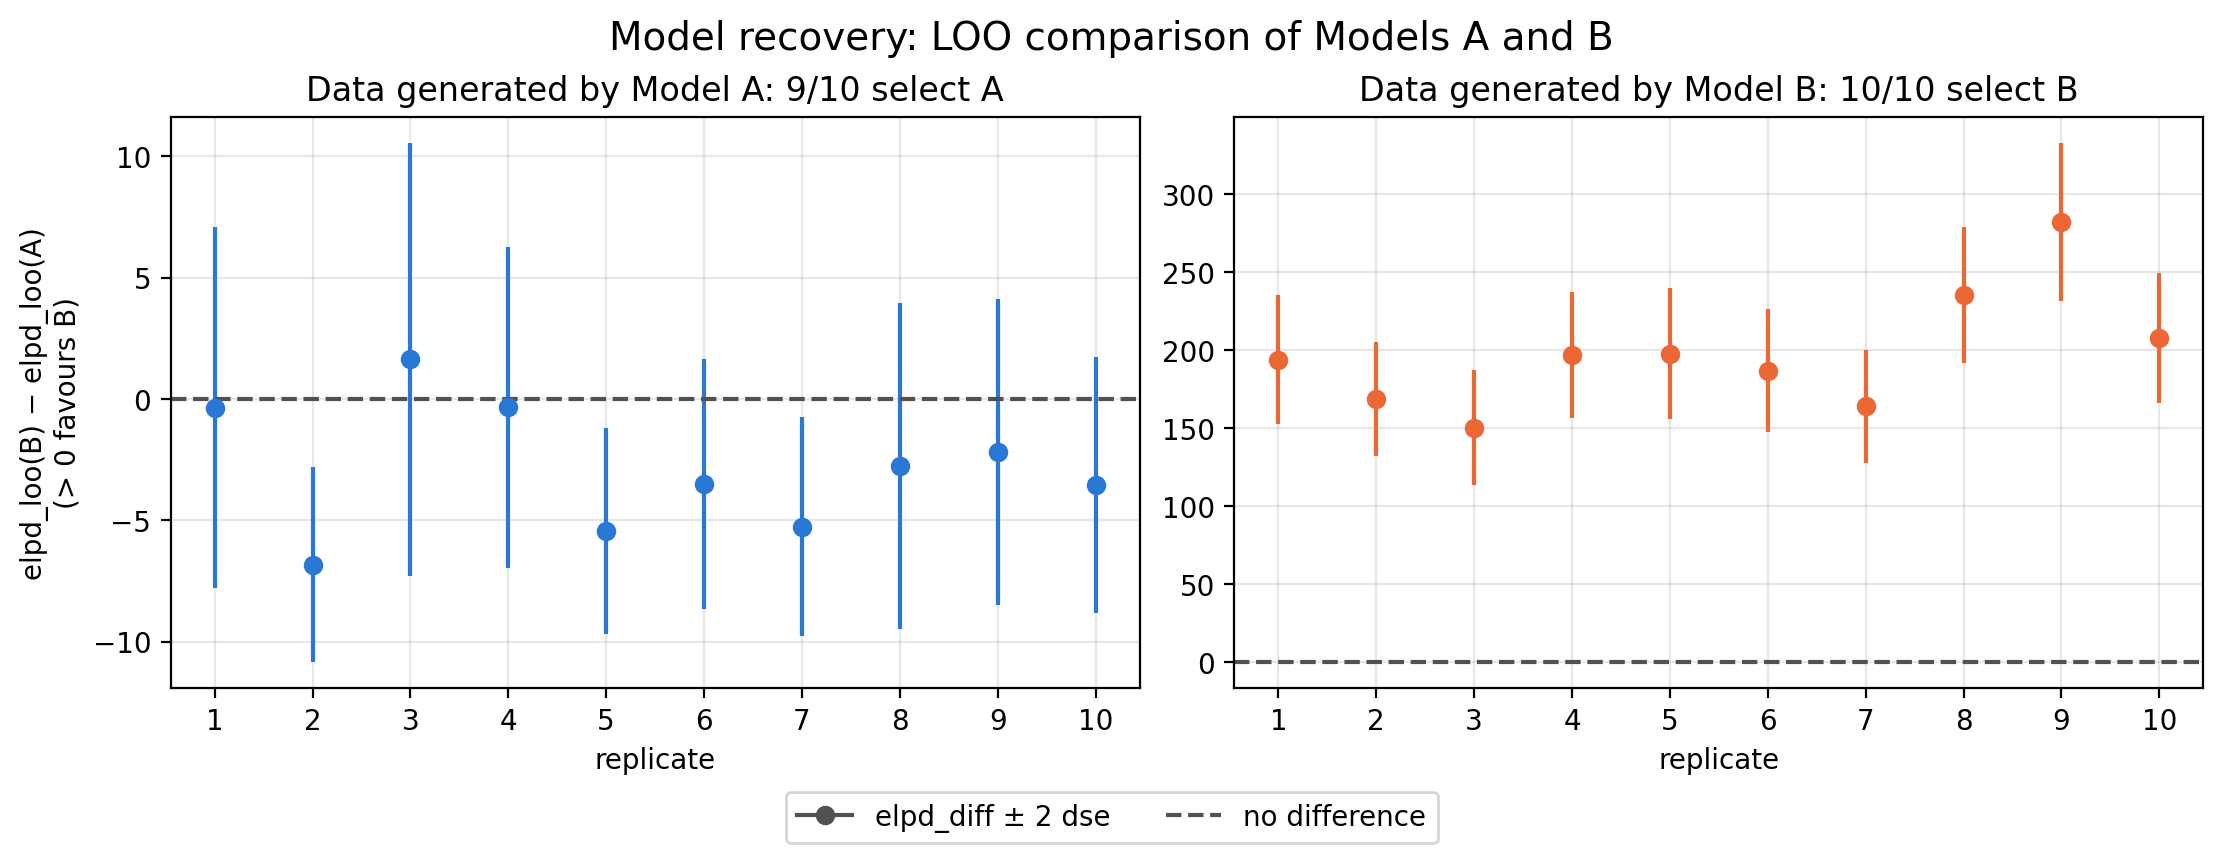
\includegraphics[width=\textwidth]{elpd_diff_by_replicate.png}
\caption{$\Delta = \elpd(\text{B}) - \elpd(\text{A})$ with $\pm 2$ dse for every
replicate. Left: data generated by Model A. Right: data generated by Model B. Note
the different vertical scales.}
\label{fig:elpd_diff}
\end{figure}

\paragraph{Data from B.} LOO selects B every time, by a wide margin: $\Delta$ ranges
from 150.2 to 282.4 (median 195.4) and $z$ from 8.16 to 11.12. Model B's effective
number of parameters $p_\text{loo}$ is 166.7--189.6, against 12.5--14.7 for A.

\paragraph{Data from A.} LOO selects A in 9 of 10 replicates, but by small margins:
$\Delta$ ranges from $-6.83$ to 1.63 (median $-3.14$), with $z$ from $-3.41$ to 0.36.
The difference is more than 2 dse in favor of A in only 3 of the 10 replicates; in the
other 7, $|z| \le 2$. The one replicate where B is selected is a near-tie
($\Delta = 1.63$, $z = 0.36$). This is the expected pattern when the true model is
the simpler one nested inside the other: B can mimic A by shrinking its
between-session sds toward 0, and then loses only the small LOO cost of its extra
flexibility. Accordingly, B's $p_\text{loo}$ on data from A is 53.9--83.6, much lower
than on data from B. The comparison is therefore asymmetric: it identifies
session-to-session variation clearly when it is there, but it cannot strongly
confirm that it is absent.

\paragraph{Real data.} The real difference, $\Delta = 164.1$ ($z = 8.55$), lies inside
the range produced by data from B (150.2 to 282.4) and far outside the range produced
by data from A ($-6.83$ to 1.63). Model B's $p_\text{loo}$ on the real data, 178.7,
also matches the data-from-B range (166.7--189.6) rather than the data-from-A range.

\section{Diagnostics}

\paragraph{Sampling.} All 40 fits sampled without divergences. Over all fits, the
maximum $\hat{R}$ is 1.004 for Model A and 1.009 for Model B, and the minimum bulk ESS
is 2411 and 857.

These $\hat{R}$ and ESS values leave out the variables $z_{\sigma}$ behind Model B's
between-session sds of $\beta_0$ and the lapse rates, which enter the model only
through an absolute value ($\sigma_{\beta_0} = |2 z_{\sigma_{\beta_0}}|$, and similarly
for $\sigma_\gamma$). Their sign is therefore not identified, and when the true sd is
clearly above 0 different chains settle on opposite signs. On data from B, their
$\hat{R}$ is 1.53--1.74, which looks like a failed fit. Nothing that enters the
likelihood depends on that sign, so the sds themselves, and everything computed
from them, are checked instead (the values above). On data from A, where the sds are
close to 0 and the two signs overlap, their $\hat{R}$ is at most 1.059.

\paragraph{LOO.} The largest Pareto $k$ over all fits is 0.645, below the 0.7 threshold
above which PSIS-LOO estimates are unreliable. No fit has a $k$ above 0.7.

\section{Conclusions}

\begin{itemize}
  \item With the real design and data of this size, LOO identifies session-to-session
        variation reliably: when it is present at the level estimated from the real
        data, B wins every time with $z > 8$.
  \item B's flexibility alone does not make it win. On data without session variation,
        B loses or ties ($\Delta$ at most 1.63), so B's advantage on the real data,
        164.1, is not something its extra parameters produce by themselves.
  \item The real-data comparison looks like the data-from-B replicates in both $\Delta$
        and $p_\text{loo}$. Taken together, the preference for Model B on the real data
        is good evidence that the psychometric curves vary between sessions.
  \item The reverse question, confirming that some form of session variation is
        absent, is answered only weakly by LOO, since the more flexible model loses
        by just a few elpd points when the simpler one is true.
\end{itemize}

\paragraph{Limitations.}
\begin{enumerate}
  \item Ten replicates per generating model: enough to see that the two
        distributions of $\Delta$ are far apart, but not to estimate an error rate
        precisely.
  \item Data from B use one set of hyperparameters, those of the real fit. With
        smaller between-session sds, the gap between the models would shrink.
\end{enumerate}

\end{document}
